%!TEX root = ../report.tex


\chapter{Implementation}\label{ch:implementation}

% TODO @all add introduction to implementation
\lipsum[2-4]


\section{Libraries}\label{sec:libraries}
% TODO rename this chapter to make clear that the libraries are self-developed
% TODO @all add introduction to libraries
% -> why libraries?
% -> advantages?
% -> disadvantages?

\subsection{Persistence}\label{subsec:persistence}

% TODO @joernneumeyer & @mauritsvanderzee
% TODO add link to npm

\subsection{Transport}\label{subsec:transport}
% TODO @joernneumeyer & @mauritsvanderzee
% TODO add link to npm

\subsection{Utilities}\label{subsec:utilities}
% TODO @joernneumeyer & @mauritsvanderzee
% TODO add link to npm


\section{Frontend}\label{sec:frontend}

\subsection{Services}\label{subsec:services}

% TODO rework introduction section
The following part of the dossier will describe the different services which have been developed during the time of the project.
This will include a description of each service, followed by an REST API specification.

\subsubsection{API Service}\label{subsubsec:api-service}

The API service is a rather small service located in the desktop client.
The service is responsible for managing the global state of all relevant API information in the desktop application.
In the current state of development this includes the following information

\begin{itemize}
    \item hostname - the hostname of the server (e.g. trale.org)
    \item port - the default port on which the service is listening for incoming connections (default: 8086)
    \item the remote endpoint - a constructed string for building a connection to the server (e.g.\ http://trale.org:8086)
    \item trale port - the default port on which the service is listening for encrypted messages (default: 8087)
\end{itemize}

Further, the service provides several helper methods for retrieving and updating the remote endpoint as well as several
getters and setters for all above mentioned attributes.

\subsubsection{Auth Service}\label{subsubsec:auth-service}
The auth service is responsible for managing authentication related tasks such as login, logout, registration and
minor helper functions (e.g.\ forgot password).

\paragraph{Login function}
The login takes a username and a password as parameters and executes a post request to the remote endpoint specified in
the \textbf{\hyperref[subsubsec:api-service]{API service}}.
On a successful login a token will be provided for future authentication, otherwise an error stating 'Invalid
credentials - Status code 400' will be returned.

% TODO @joernneumeyer maybe add register / logout etc. here as well? refactor code? not in auth service yet

Due to the mentioned responsibilities, this service is only injected in authentication related components.

\subsubsection{Contact Service}\label{subsubsec:contact-service}

The contact service is responsible for managing all contact related tasks and corresponding state management.
It owns a contact array holding all contacts for the currently logged-in user.
On application startup the contact service will load all contacts from drive by utilizing the
\textbf{\hyperref[subsubsec:crypto-storage-service]{Crypto Storage Service}}.

Besides providing a loading wrapper for retrieving encrypted contacts from the drive it also manages actions such as
adding contacts, updating contacts or fetching the latest message of all contacts to display those in the contact list.

Lastly, the contact service provides a function to load the actual chat of a specific contact with the currently
logged-in user.

% TODO @joernneumeyer any additional remarks / information to be added?

\subsubsection{Debug Service?}
% TODO @joernneumeyer & @mauritsvanderzee
% @joernneumeyer shall we include debug service?

\subsubsection{Crypto Storage Service}
% TODO @joernneumeyer & @mauritsvanderzee

\subsubsection{Key Registry Service}
% TODO @joernneumeyer & @mauritsvanderzee

\subsubsection{Titp Service}
% TODO @joernneumeyer & @mauritsvanderzee

\subsubsection{Util Service}
% TODO @mauritsvanderzee

\subsection{Components}

\subsubsection{Admin Panel}

\paragraph{Security Setting}
The Security Settings component gives the admins of the SocialStuff server the possibility to change the behaviour of the SocialStuff server
regarding the security standards. The user can change the settings and send them to the backend via the settings service in the gateway.
These settings influence other functions depending on the current settings.
\begin{figure}[h]
    \centering
    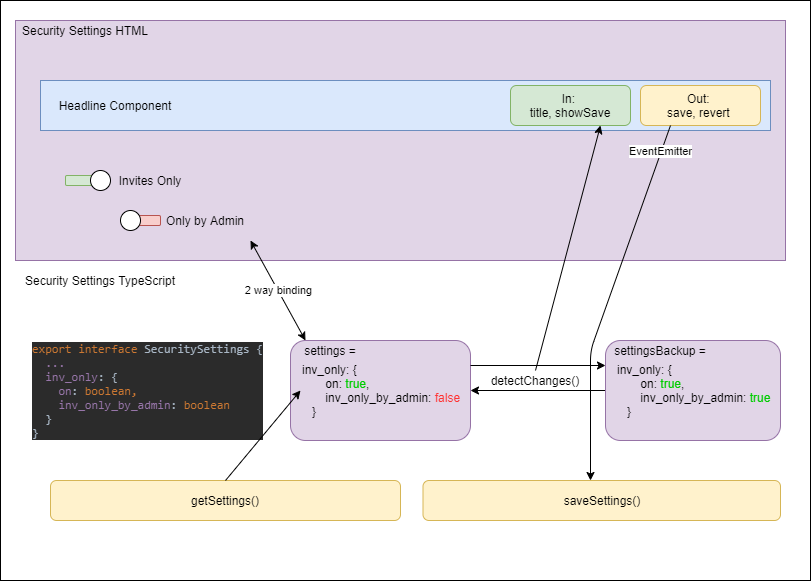
\includegraphics[width=1.0\textwidth]{./images/security_settings}
    \caption{Visualisation of the security-settings component}
    \label{fig:secset}
\end{figure}
The HTML contains the headline component and a lot of switch buttons. The headline component is given two attributes,
a title as a string and a Boolean called "showSave". The headline component also has two output events called "save" and "revert".
The TypeScript file (.ts file) of the Security Settings component loads a SecuritySettings object (the corresponding interface can be found in the folder "admin/interfaces") with the function getSettings (l. 41 - 50).
This function retrieves the current settings from the server via the settings service of the admin panel (folder "services").
\begin{itemize}
    \item You can find a brief explanation about how all services in Angular acts inside the \hyperref[subsec:services]{\textbf{services}} chapter
\end{itemize}
The received SecuritySettings object is then stored simultaneously in two attributes "settings" (l. 22) and "settingsBackup" (l. 22).
All buttons are bound to the SecuritySettings object containing the attribute "settings" via the expression "[(ngModel)]".
If you change the value of one of the switch buttons, you will see that the headline module displays two buttons "Save" and "Reset. /newline As mentioned earlier, the headline component has an input directive called "show save". This controls whether the "Save" and "Reset" buttons are displayed or not. The passed attribute, is a computed attribute (l. 33). A computed attribute is a mixture of attribute and method. It is seen as an attribute by the invoker, but it consists of two methods, a getter and a setter method. In our case, only one getter method is defined.
It uses the function "isEqual" from the installed package "lodash".
\begin{itemize}
    \item You can find the full documentation of lodash under: https://lodash.com/docs/4.17.15
\end{itemize}
The moment changes are made via the switch buttons, the attribute settings also change. The calculated attribute "isEqual" is then changed from false to true. This causes the headline component to display the "Save" and "Reset" button. When the user presses a button, the headline component sends an event to the Security Settings component that triggers the call of the Save or Revert function. \\
The save function calls a function within the admin panel settings service that sends a "PUT" request to the endpoint.
The revert function clones the SecuritySettings object from the settingsBackup attribute into settings, undoing any changes made without saving.

\paragraph{Report Settings}
This feature includes a reporting system. Users of our web application can report each other, which makes it possible to detect users who violate the rules set by the administrators. In the administration interface, it is possible to change the settings of the current reporting system and turn it on or off. This feature also offers the possibility to add, edit or delete report reasons. Each ReportReason (finadable in admin/interfaces) has three fields:
\begin{verbatim}
export interface ReportReason {
  id: string;
  reason: string;
  max_report_violations: number;
}
\end{verbatim}
The parent component and the entry for the whole feature is the report-settings component.
\begin{figure}[h]
    \centering
    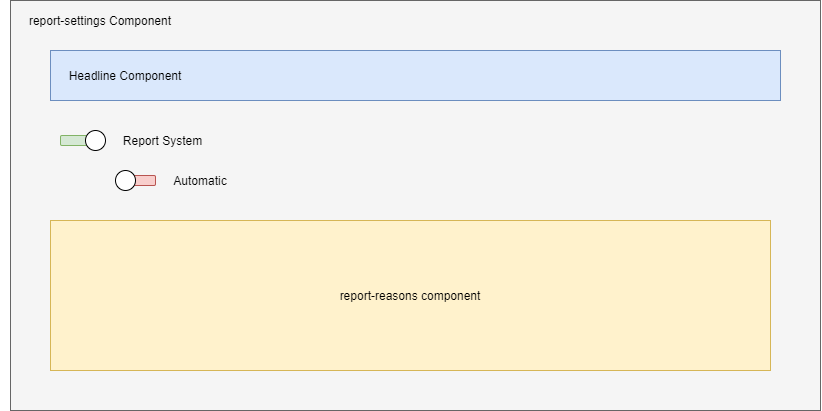
\includegraphics[width=1.0\textwidth]{./images/report_settings_1}
    \caption{Visualisation of the report-settings component}
    \label{fig:reportset}
\end{figure}
\\
For this component only the HTML file is visualized because there is nothing important going on inside the TypeScript file of this component. The HTML includes the headline component which shows the title of this feature and is used in all of the features of the admin panel. Next to the headline component two switch buttons are shown. At the moment these Buttons have no influence and are just bind to a dummy attribute. The creating, editing and deleting of report reasons are done in the embedded report-reasons component.
\begin{figure}[h]
    \centering
    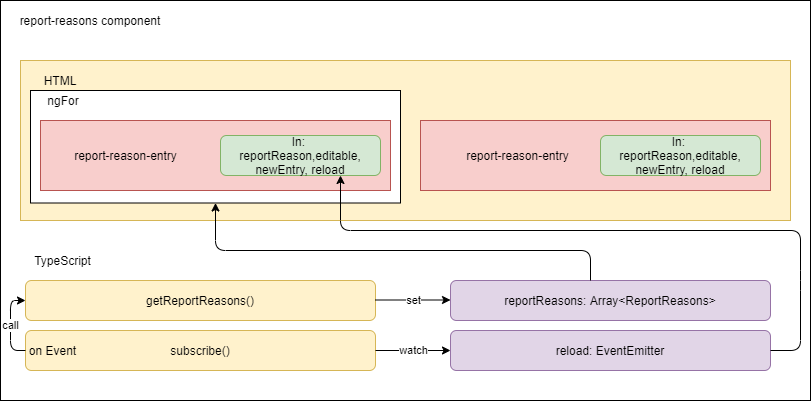
\includegraphics[width=1.0\textwidth]{./images/report_reasons_2}
    \caption{Visualisation of the report-reasons component}
    \label{fig:reportreason}
\end{figure}
\vspace{5mm}
\\
The report-reasons component is responsible for showing all report reasons previously created. They are loaded with the method getReportReason and stored inside the variable reportReasons. Through this array the ngFor Method itterates, embedding for each ReportReason Object inside the array a report-reason-entry component inside the HTML. The TypeScript File holds a second variable called “reload”. Here an instance of a new EventEmitter is created. An EvenEmitter is used to emit custom events synchronously through multiple components and register handlers for those events by subscribing to the instance. The reload instance is passed via the Input directive to the report-reason-entry and via the subscribe method, emits can be detected. If any emit is done inside another component holding the same instance, the getReportReasons function is called which will lead to an update of the Array of ReportReasons. This is important to trigger an update as soon as a report reason has been edited. Next to the ngFor loop the the HTML file embeds another report-reason-entry component and passing over the input directive “newEntry” a true. This will change the behaviour of the component so that it can be used to create a new report reason.
So now we have a list of all report reasons and the possibility to add a new one. Next, it will be explained how
the report-reason-entry component works.
\begin{figure}[h]
    \centering
    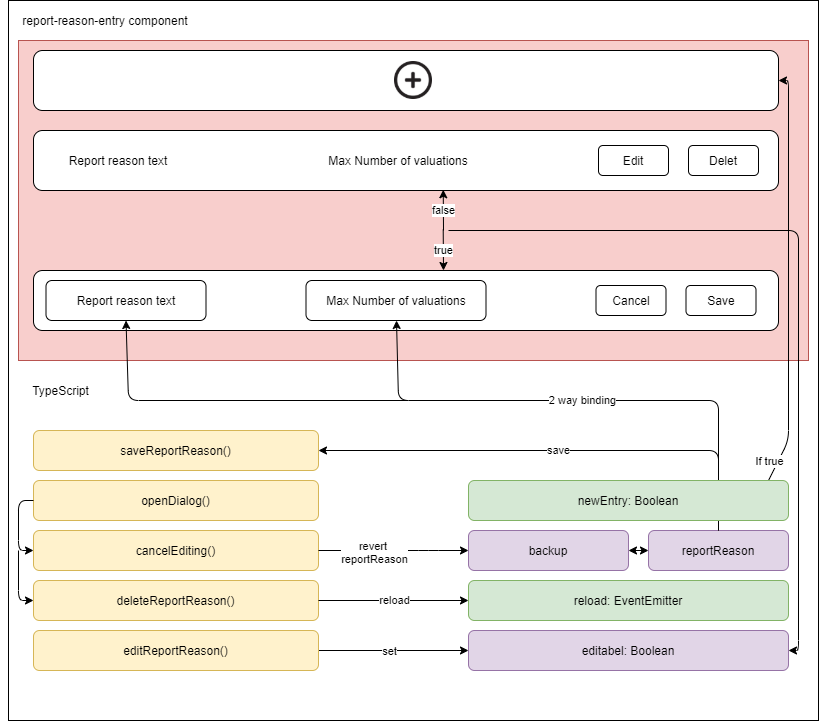
\includegraphics[width=1.0\textwidth]{./images/report_reason_entry_3}
    \caption{Visualisation of the report-reason-entry component}
    \label{fig:reportreasonent}
\end{figure}
\vspace{5mm}
\\
The report-reason-entry component can act in three different ways based on the variable “editable” and the input directive “newEntry” inside the TypeScript file of the component. If the component got a “true” via the input directive, the HTML is showing a button to add a new entry. By clicking the button the function editReportReason() is called and the variable editable is set to “true”. This change will again trigger the HTML to change its appearance showing two text fields, a save and a cancel button. If neither of those two variables is set to true the component just shows the report reason text, the number of valuations, an edit, and a delete button. The delete button does not trigger the deleteReportReason method, but the openDialog method, which embeds a confirmation dialogue warning the user that the deletion cannot be undone. For this dialogue, we used a pre-built UI component from Angular Material (found in the technology stack). Only when the user confirms the decision, the deleteReportReason method is called. If the deletion was successful, an event is emitted via the instance "reload".
This triggers a reload within the parent component. While editing or creating a new reason the users can either save or cancel their changes. When the "Save" button is pressed, all changes are sent to the server and are persisted in the database. An event is only emitted when a new reason has been created. If an existing reason has been edited, there is no need to do a reload within the parent component. Calling the "cancelEditing" method causes the variable reportReason to be reset to the state before editing and the variable
"editable" to be set to false.

\paragraph{Reported Users}
The graphical user interface for displaying all reported users is completed and can be found in the folder "ReportSystem/ReportedUsers".
There you will find a total of 4 components for creating the list that displays all reported users.
\\
\begin{figure}[h]
    \centering
    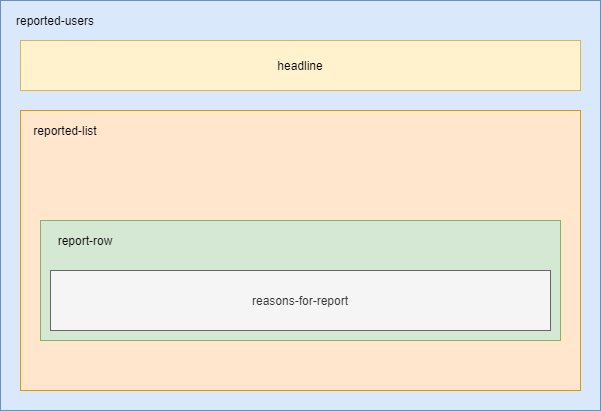
\includegraphics[width=1.0\textwidth]{./images/report_component}
    \caption{Visualisation of the reported-users component}
    \label{fig:reportedusers}
\end{figure}
\\
\begin{enumerate}
\item Reported-users
   \begin{itemize}
     \item This is the parent component just includes the headline and the report-list component.
   \end{itemize}
\item Report-list
   \begin{itemize}
        \item Includes a table with the labels “Username” and “Times Reported”. The table rows are loaded with ngFor over a next component called report-row. Currently the data for the reported users is dummy data generated in the TypeScript file of this component. Here it is still need to embed a function, retrieving all reports from the endpoint. (Use the gateway and create a service in the “services” folder) In the end you need an array of userReport objects (You find the interface for those objects already in the folder “admin/interfaces”). Iterate through this array with ngFor and pass the current userReport to the report-row component.
   \end{itemize}
\item Report-row
   \begin{itemize}
       \item This component shows all information regarding a userReport. When clicking the dropdown icon, the row will expand, showing all reasons the report reason includes. (line 6-11) This is done by another component which gets as an input
       directive an array of all the reasons connected to the reportReason.
   \end{itemize}
\item Reasons-for-report
   \begin{itemize}
      \item This is a simple component iterating through all the reasons passed.
      It contains two functions, one computed function for retrieving the highest number of all reportReasons (l. 18-24) and a function retrieving a string (‘ok’, ‘low’, ‘middle’ or ‘high’) based on the percentage towards the highest number retrieved by the computed function. The string is attached to the class name “times-reported” (html-file, l.4) and regulates the color of the number.
   \end{itemize}
\end{enumerate}

\paragraph{Create Invite}
This feature includes two main component, which again are splitted up in smaller components.

\begin{enumerate}
\item invite-code-list
	\begin{itemize}
		\item This Component holds the table with all existing invite codes. It is responsible for loading all entries from the back-end through the function getInviteCodes from the Gateway and presenting them in a table. The component iterates through all entries and passing the data of each entry towards another component presenting a row in the table. The Component has as input an EventEmitter to pass it towards the InviteCodeRow component, making it possible to trigger the getInviteCodes function after deleting an InviteCode from the InviteCodeRow component and update the data.
	\end{itemize}
\item create-new-invite
	\begin{itemize}
		\item This Component holds the functionality to create a new InviteCode and save it on the server. It has three fields: \\  
		\textbf{1.	Expiration Date:} This field uses the ngx-mat-datetime package which adds the functionality of not choosing just a date but also a time. \\
		\textbf{2.	Usage Limitation:} A number indicating how often the invite code can be used. Optional, default is 0 and specify that the invite code has no usage limitation. \\
		\textbf{3.	Invite Code:} A string which will be used when register onto the platform. A 10-character-long string (numbers and uc characters) can be generated using the generate button.\\	
	\end{itemize}	
\end{enumerate}

\section{Backend}

\subsection{Database Connections}

\subsection{Services}

\subsubsection{Authentication Service}
% TODO @joernneumeyer

\subsubsection{File Service}
% TODO @all shall we just briefly mention that this might be a service for future features / development

\subsubsection{Identity Service}
\label{subsubsec:identitySer}
% TODO @joernneumeyer

\subsubsection{Settings Service}\label{subsubsec:settingsSer}

The Settings service provides an interface to the admin panel frontend and carries out the settings to the other
services.
This service was developed in parallel to the admin panel frontend. %TODO @maltecastner insert reference to component, once it has been added
First only the for the UI necessary functionality would be added, later on the actual functionality was added
(e.g.\ that users can actually be reported for the report reasons added in the settings).
As it can be seen from the use case diagram~\ref{fig:ucd} the settings service carries out a few tasks by itself whilst
forwarding certain other requests to the \hyperref[subsubsec:identitySer]{\textbf{identity service}} and the
\hyperref[subsubsec:reportingSer]{\textbf{reporting service}}.
The use cases as well as their descriptions are located in the
\hyperref[ch:software-requirements-specification-(srs)]{\textbf{\ac{srs}}}

\begin{figure}[!ht]
    \centering
    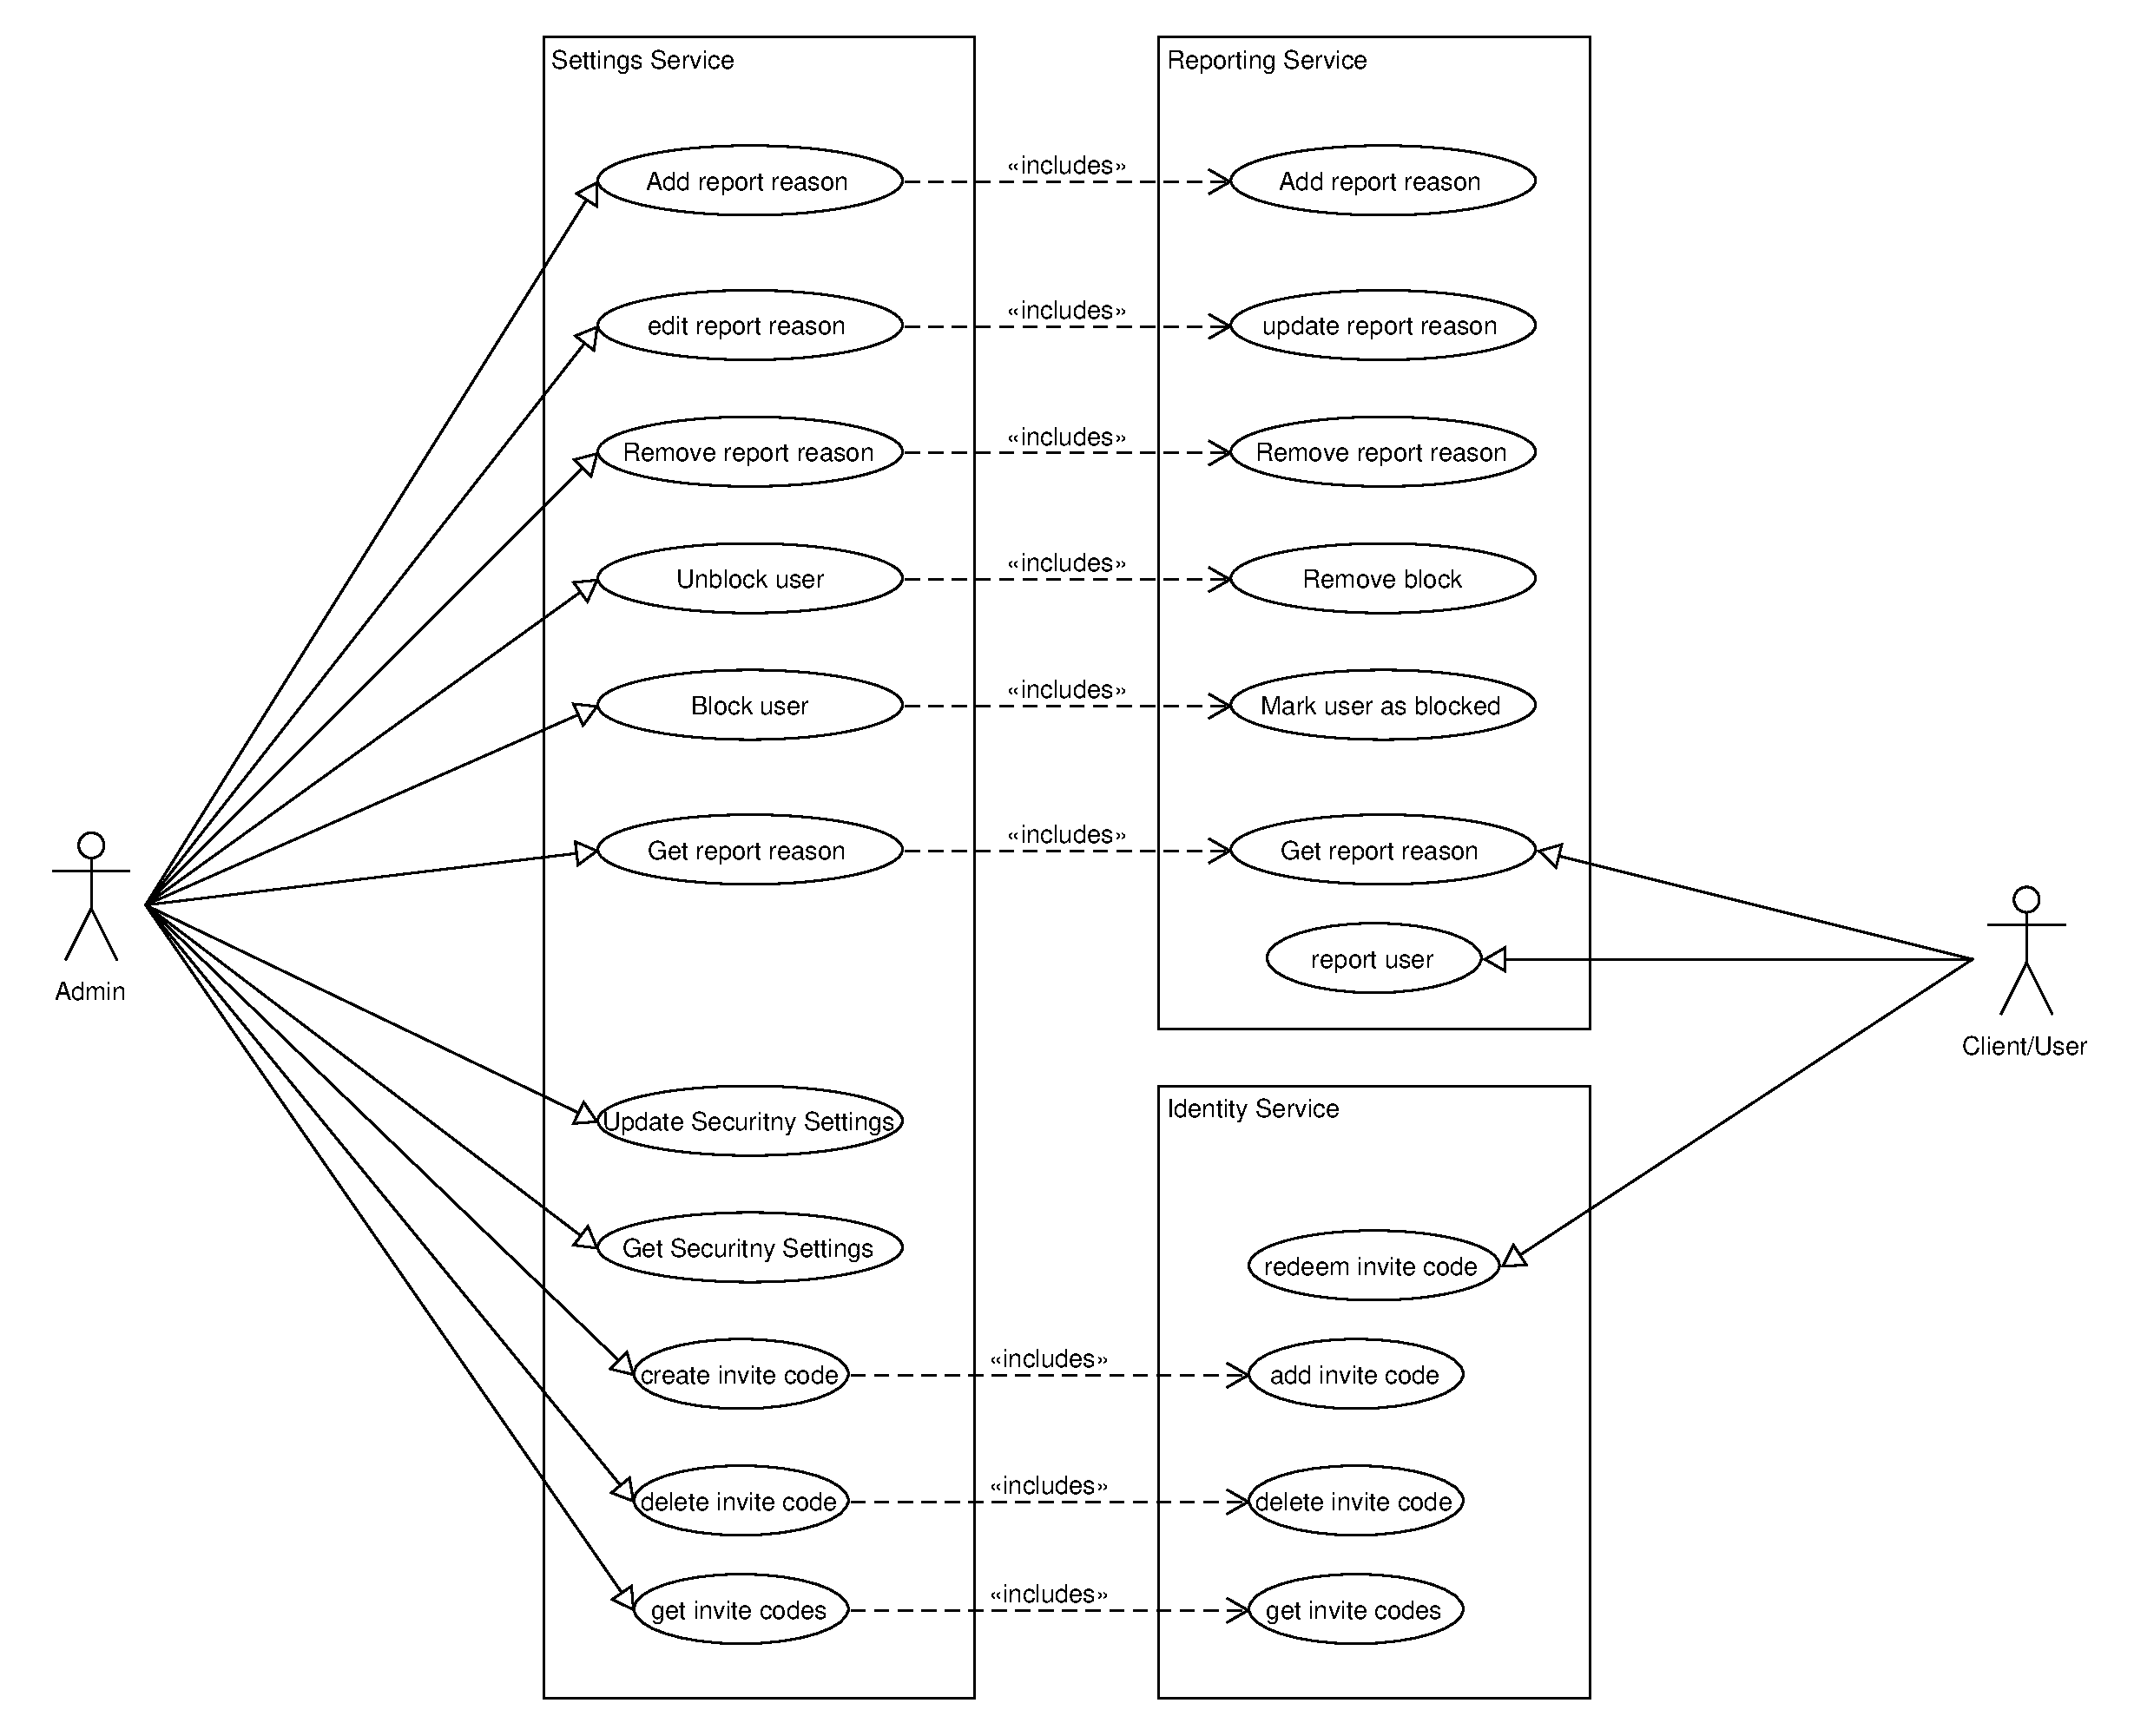
\includegraphics[width=1.0\textwidth]{./images/UseCaseDiagramAdminPanel}
    \caption{Use case diagram of the admin panel showing responsibility of each AP service}
    \label{fig:ucd}
\end{figure}

\paragraph{Rest interface}

The settings service provides the following rest endpoints:

\begin{lstlisting}[label={lst:lstlisting}]
GET: /settings/report-reason
\end{lstlisting}

Returns all report reasons as a JSON array.

\begin{lstlisting}[label={lst:lstlisting2}]
POST: /settings/report-reason
body:
{
"reason": "some reason",
"max_report_violations": 5
}
\end{lstlisting}

Adds a new report reason.

\begin{lstlisting}[label={lst:lstlisting3}]
PUT: /settings/report-reason
body:
{
"id": 123,
"reason": "some reason",
"max_report_violations": 5
}
\end{lstlisting}

Edits an existing report reason.

\begin{lstlisting}[label={lst:lstlisting4}]
DELETE: /settings/report-reason
headers:
- "id": 123
\end{lstlisting}

Deletes a report reason with an id that is provided as a header.

\begin{lstlisting}[label={lst:lstlisting5}]
GET: /settings/security
\end{lstlisting}

Returns the current security settings.

\begin{lstlisting}[label={lst:lstlisting6}]
PUT: /settings/security
body:
{
    "two_factor_auth": {
    "on" : true,
    "phone": false,
    "email": true
},
    "confirmed_emails_only": true,
    "individual_pwd_req": {
    "on": true,
    "upper_case": true,
    "number": true,
    "special_char": true,
    "reg_ex": false,
    "reg_ex_string": "[]"
},
    "inv_only": {
        "on": false,
        "inv_only_by_adm": false
    }
}
\end{lstlisting}

Edits the security settings.
The new settings are provided in body.

\paragraph{Example add report reason}

\begin{figure}[!ht]
    \centering
    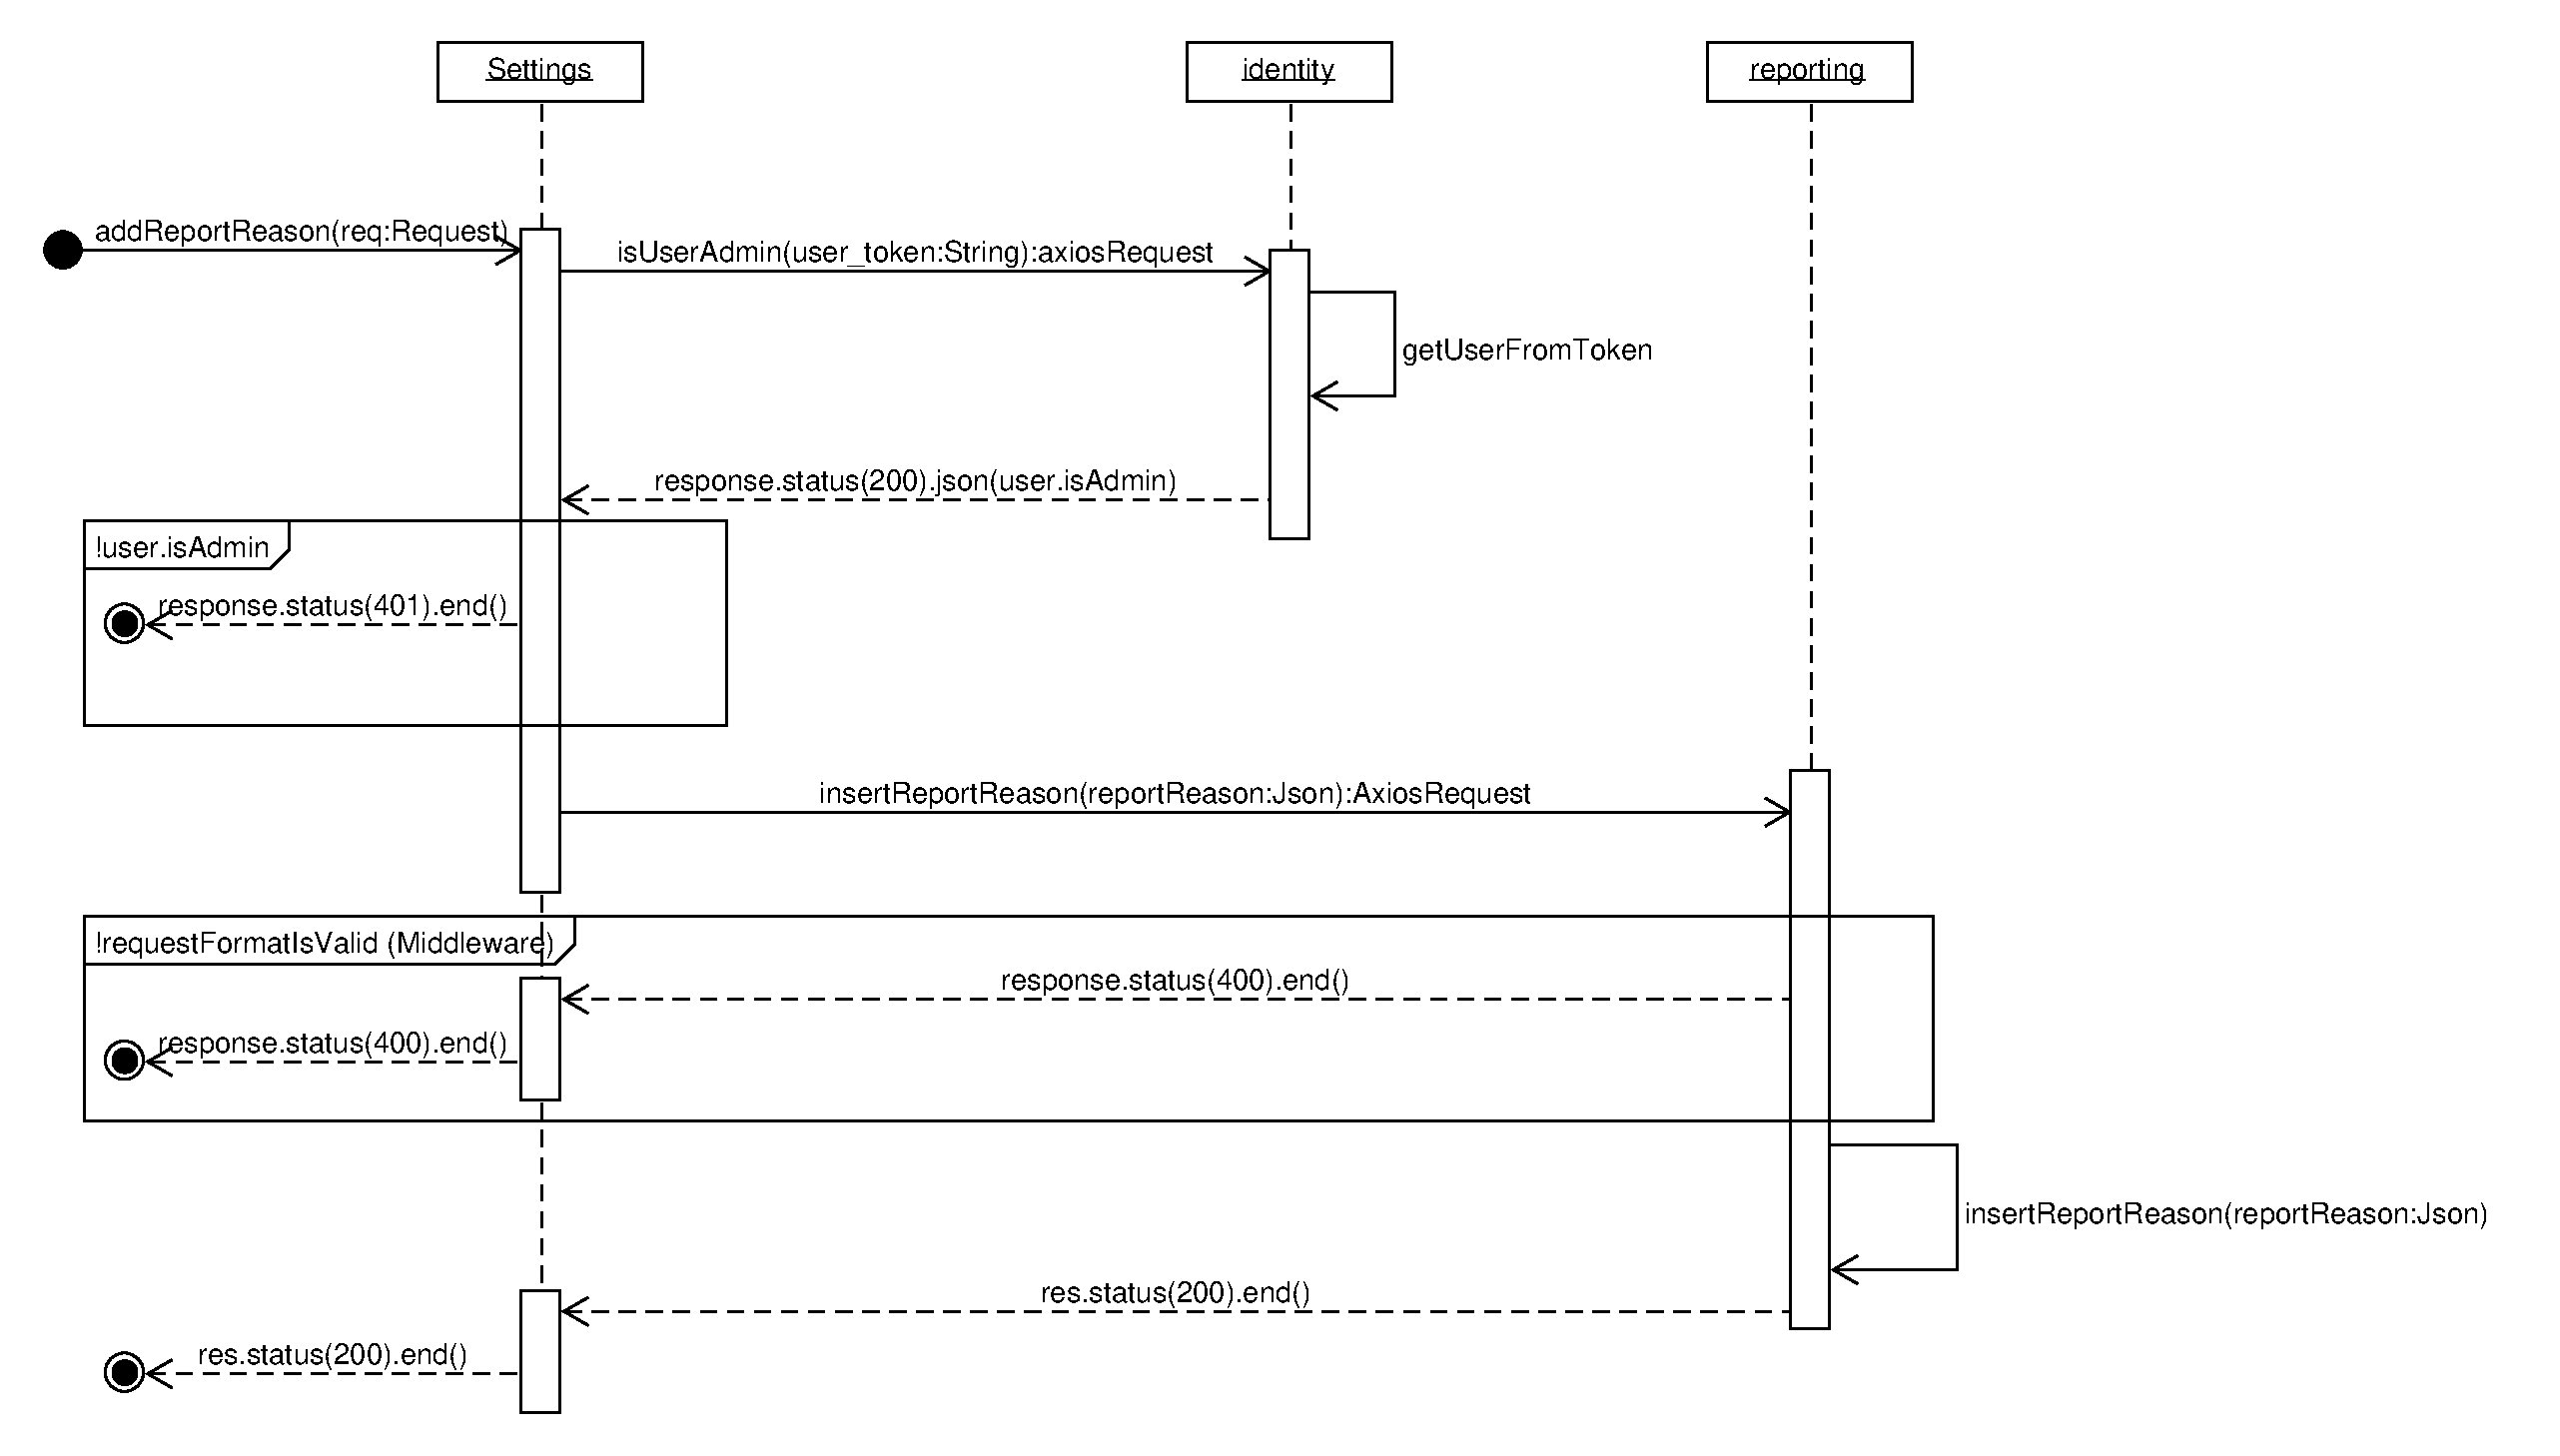
\includegraphics[width=1.0\textwidth]{./images/SequenceDiagram_AddReportReason}
    \caption{Use case diagram of the admin panel showing responsibility of each AP service}
    \label{fig:addReportReason}
\end{figure}

The sequence diagram~\ref{fig:addReportReason} shows an example of the communication of the settings service with the
aforementioned services.
The event is triggered by a request from the client.
Firstly the settings service will be verifying the identity of the sender by checking at the identity service, if the
user who sent out the request is in fact an administrator.
Then the request will e forwarded to the reporting service.
Here it will be checked if the request format is valid.
Should this not be the case, the reporting service will return an error (status 400).
Otherwise, the reason will be added in the reporting database, which will then be returned to the settings service,
who will then let the client know by response that the insertion was a success.
This way each service has a clearly defined task.

\subsubsection{Reporting Service}\label{subsubsec:reportingSer}

The reporting service handles the reporting system.
This includes administrative tasks like managing for which reasons users can be reported, as well as the reporting
system itself (reporting users and banning them).
The administrative tasks, like adding new report reasons, manually blocking and unblocking users, can be done via the
\hyperref[subsubsec:settingsSer]{\textbf{settings service}}.
This service was added in the later stages of the project.

First the entire reporting was handled via the \hyperref[subsubsec:settingsSer]{\textbf{settings service}}, however it
was decided that the reporting itself should possess its own service. % TODO @tobiasjansen --> why? explanation missing
Therefore, it was necessary to outsource the report related functionality from the
\hyperref[subsubsec:settingsSer]{\textbf{settings service}} to the
\hyperref[subsubsec:reportingSer]{\textbf{reporting service}}.

\paragraph{Rest Interface}
\begin{lstlisting}[label={lst:lstlisting7}]
POST: /report-reasons
body:
{
    "reason": "some reason",
    "max_report_violations": 5
}
\end{lstlisting}

Adds a new report reason returning the ID of the added report reason.

\begin{lstlisting}[label={lst:lstlisting8}]
PUT: /report-reasons
body:
{
    "id": 12
    "reason": "some reason",
    "max_report_violations": 5
}
\end{lstlisting}

Edits a report reason by the \enquote{ID} key and returns the edited reason.

\begin{lstlisting}[label={lst:lstlisting9}]
GET: /report-reasons
\end{lstlisting}

Returns all existing report reasons as JSON array

\begin{lstlisting}[label={lst:lstlisting10}]
DELETE: /report-reasons
headers
    - id: 12
\end{lstlisting}

Deletes a report reason by ID which is provided in the header of the request.
Returns the ID of the deleted request in its body.

\begin{lstlisting}[label={lst:lstlisting11}]
Headers:
    - user_token
Body:
{
    "username": "userHashOfUserBeingReported",
    "reason_id": 123
}
\end{lstlisting}

Reports a user based of the report reason, and the users' username hash.
A user can only be reported by the same user for the same reason after 15 minutes to prevent spamming.
Otherwise, the report will be processed by the backend, and the user will be set to \enquote{blocked} in case one
exceeds the maximum report violation counter.

